%!TEX root = ../main.tex
\doublespacing
\chapter{Observations of Radio Scattering in the Solar Corona compared to Computational Modelling.}
\label{chap:observations_vs_theory}
Recent developments in the modelling of radio waves in a turbulent corona have made predictions about source sizes that have not yet been qualitatively compared to interferometric observations. Scattering of radio waves off of density inhomogeneities in the solar corona is considered to be the dominant cause of the size and shape of radio bursts. By understanding scattering, the turbulent nature of processes that generate density inhomogeneities can be studied. Turbulence in the corona can give insight into how energy is transferred from large scale phenomena down to the microscales resulting in the million degree Kelvin temperatures that have puzzled solar physicists for decades. New models of radio wave scattering, therefore, are the first step to solving fundamental physical problems in the solar corona. However, unless the models agree with observations, their use is limited at best and as such, comparisons between models and observations are crucial. In this chapter I utilise the direct visibility fitting method described in Chapter \ref{chap:measuring_source_sizes} and apply it to 30 Type III radio bursts. It is found that these bursts have a mean size along the major and minor axis of FWHM\textsubscript{x} = 16.35 arcmin and FWHM\textsubscript{y} = 11.86 arcmin respectively. No trend of source size with respect to helioprojective angle is found, which is in direct contrast to predictions from modelling if the intrinsic size of a burst is a point source and the degree of anisotropy is high $\alpha \sim 0.3$. This study suggests that although many are in agreement, further exploration of the parameters of scattering simulations are necessary before they can be used to predict the nature of coronal density inhomogeneities.

\section{Introduction}
\label{sec:obsvtheory_intro}
The computational modelling of radio wave scattering has seen considerable development over the 50-odd years since some of the first simulations by e.g. \cite{Fokker1965} and \cite{Steinberg1971}. The theory for these early works followed from a generalisation of \cite{Chandrasekhar1952}, as was discussed in Chapter \ref{chap:theory}, and made predictions radio burst source size, position, directivity and time profile. These works considered scattering of radio photons off of density inhomogeneities in the solar corona and considered many small angle scatterings before a final image was produced. \cite{Thejappa2007} further investigated the source directivity (power received from source in some solid angle compared to power from an isotropic source in the same solid angle) and time profiles of bursts using an updated correlation of isotropic density inhomogeneities. Initially, the inhomogeneities were assumed to have a gaussian power spectrum however, it was soon realised that they should have a Kolmogorov power spectrum of 11/3. Further study by \cite{Coles1989} and \cite{Bastian1994} of the density inhomogeniety power spectrum saw that this power scaling is only observed within a range of scales bookended by and inner and outer scale. Comparisons between these models has also been a key part in the progression of the field. \cite{Stewart1972} compare the observed positions of fundamental and harmonic emission and relate it to the then contemporary scattering models \citep[e.g.][]{Fokker1965,Steinberg1971,Riddle1974}. More recently, \cite{Krupar2020} use the model of \cite{Thejappa2007} to compare the time profiles of observed radio bursts from Parker Solar probe.


The latest development in the modelling of radio wave scattering is by \cite{Kontar2019}. Rather than using the small scattering angle approximation of previous work, \cite{Kontar2019} build on the work of \cite{Arzner1999} and \cite{Bian2019} which allows for a continuous transition from weak to strong scattering. In this approach, the effect of anisotropic density inhomogeneities is treated as photon diffusion in momentum space and the Hamiltonian equations for photon position and momentum can be solved iteratively to trace a photon's path. \cite{Kontar2019} assume a spherically symmetric corona with an anisotropic distribution of electron density fluctuations (with wavenumber $\mathbf{q}$) such that $q_\parallel$ is parallel to the local radial direction. They perform Monte Carlo simulations of photons emitted from a point source at $\omega = 1.1 \omega_p(R_s)$ via fundamental plasma emission at a distance $R_s$ and an electron density from the \cite{Parker1960} density model of a spherically symmetric corona with constant temperature. The image and time profile of each burst was found by recording the arrival of each photon at some distance where scattering is considered negligible.

For a radio burst that would be observed at $\sim 35$ MHz ($f_p = \omega_p/2 \pi \sim 32$ MHz) \cite{Kontar2019} find that an anisotropy factor of $\alpha = 0.3$ is necessary to explain observations of burst decay times.  The effect of source location on the modelled image are also investigated and it is found that sources appear more elongated in the y direction close to the disk limb and almost circular at disk centre.  This effect is less evident when an anisotropy factor of $\alpha = 0.5$ is considered. Whether this relationship is observed for Type III radio bursts located at many points along the solar disk can give a certain amount of validation to recent modelling efforts. In the following sections I describe how the size of the burst in the major and minor axes (FWHM\textsubscript{x} and FWHM\textsubscript{y} respectively) are determined from LOFAR observations and how their ``aspect ratio" i.e FWHM\textsubscript{x}/FWHM\textsubscript{y}, can be used to compare the observations with recent modelling simulations.

\section{Method}
\label{sec:obsvtheory_method}
By fitting their interferometric visibilities as described in Chapter \ref{chap:measuring_source_sizes}, the size and position of 30 Type III radio bursts over the period of 04 April 2019 to 14 April 2019 were found. The bursts were identified in LOFAR beamformed observations and their peak time determined using an automatic peak finding algorithm. Figure \ref{fig:dynamic_spectrum_070419} shows the automatically identified bursts at 30 MHz. In total, 320 bursts were identified in this way. Unfortunately, due to the strength of these bursts, the calibration of interferometric data failed for $\sim 90 \%$ of them. 30 bursts were identified manually as having successfully been calibrated and their properties fit. As well as determining the source shape and position at its peak, the area of the source over its duration was also measured. This was done by fitting a straight line to the source area over the duration of the burst, which was estimated to be 1 second before its peak and 2 seconds afterwards.

\begin{figure}[ht]
\centering
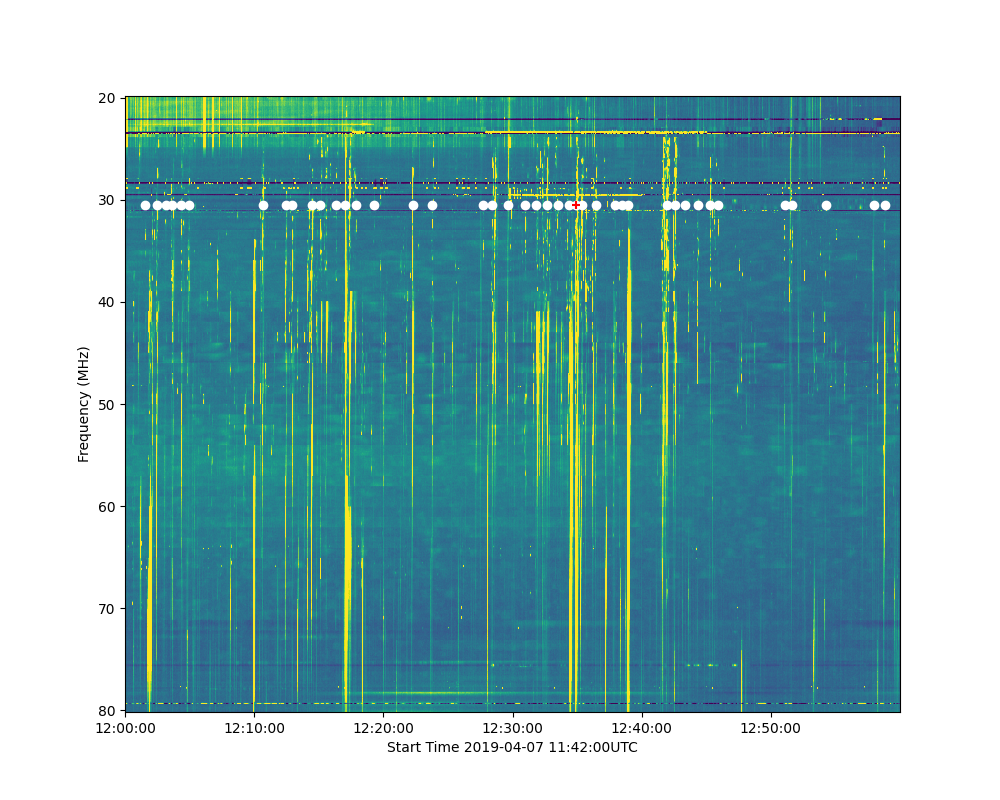
\includegraphics[width=\columnwidth]{peak_times_30MHz_2019-04-07T120000_130000.png}
\caption[Dynamic spectrum of Type III storm on 07 April 2019.]{Dynamic spectrum of Type III storm on 07 April 2019. The white dots indicate the bursts identified by an automatic peak finding algorithm, the red cross indicates the brightest burst.}
\label{fig:dynamic_spectrum_070419}
\end{figure}

\section{Results}
\label{sec:obsvtheory_results}
The parameters for all 30 fitted bursts are given in Table \ref{tab:dataset} where $I_0$ is the maximum intensity of the burst, $x_0$ and $y_0$ are the x and y  helioprojective coordinates of the burst, FWHM\textsubscript{x} and FWHM\textsubscript{y} are the burst sizes in the x and y direction and $\theta$ is the position angle of the fitted Gaussian.  Each fitted type III burst is overlayed on a synoptic AIA 193\AA  map in Figure \ref{fig:synoptic_bursts}. It is clear from the figure that most bursts share a similar size and aspect ratio despite their relatively widespread origin in relation to the Sun's disk.

\begin{figure}[ht]
\centering
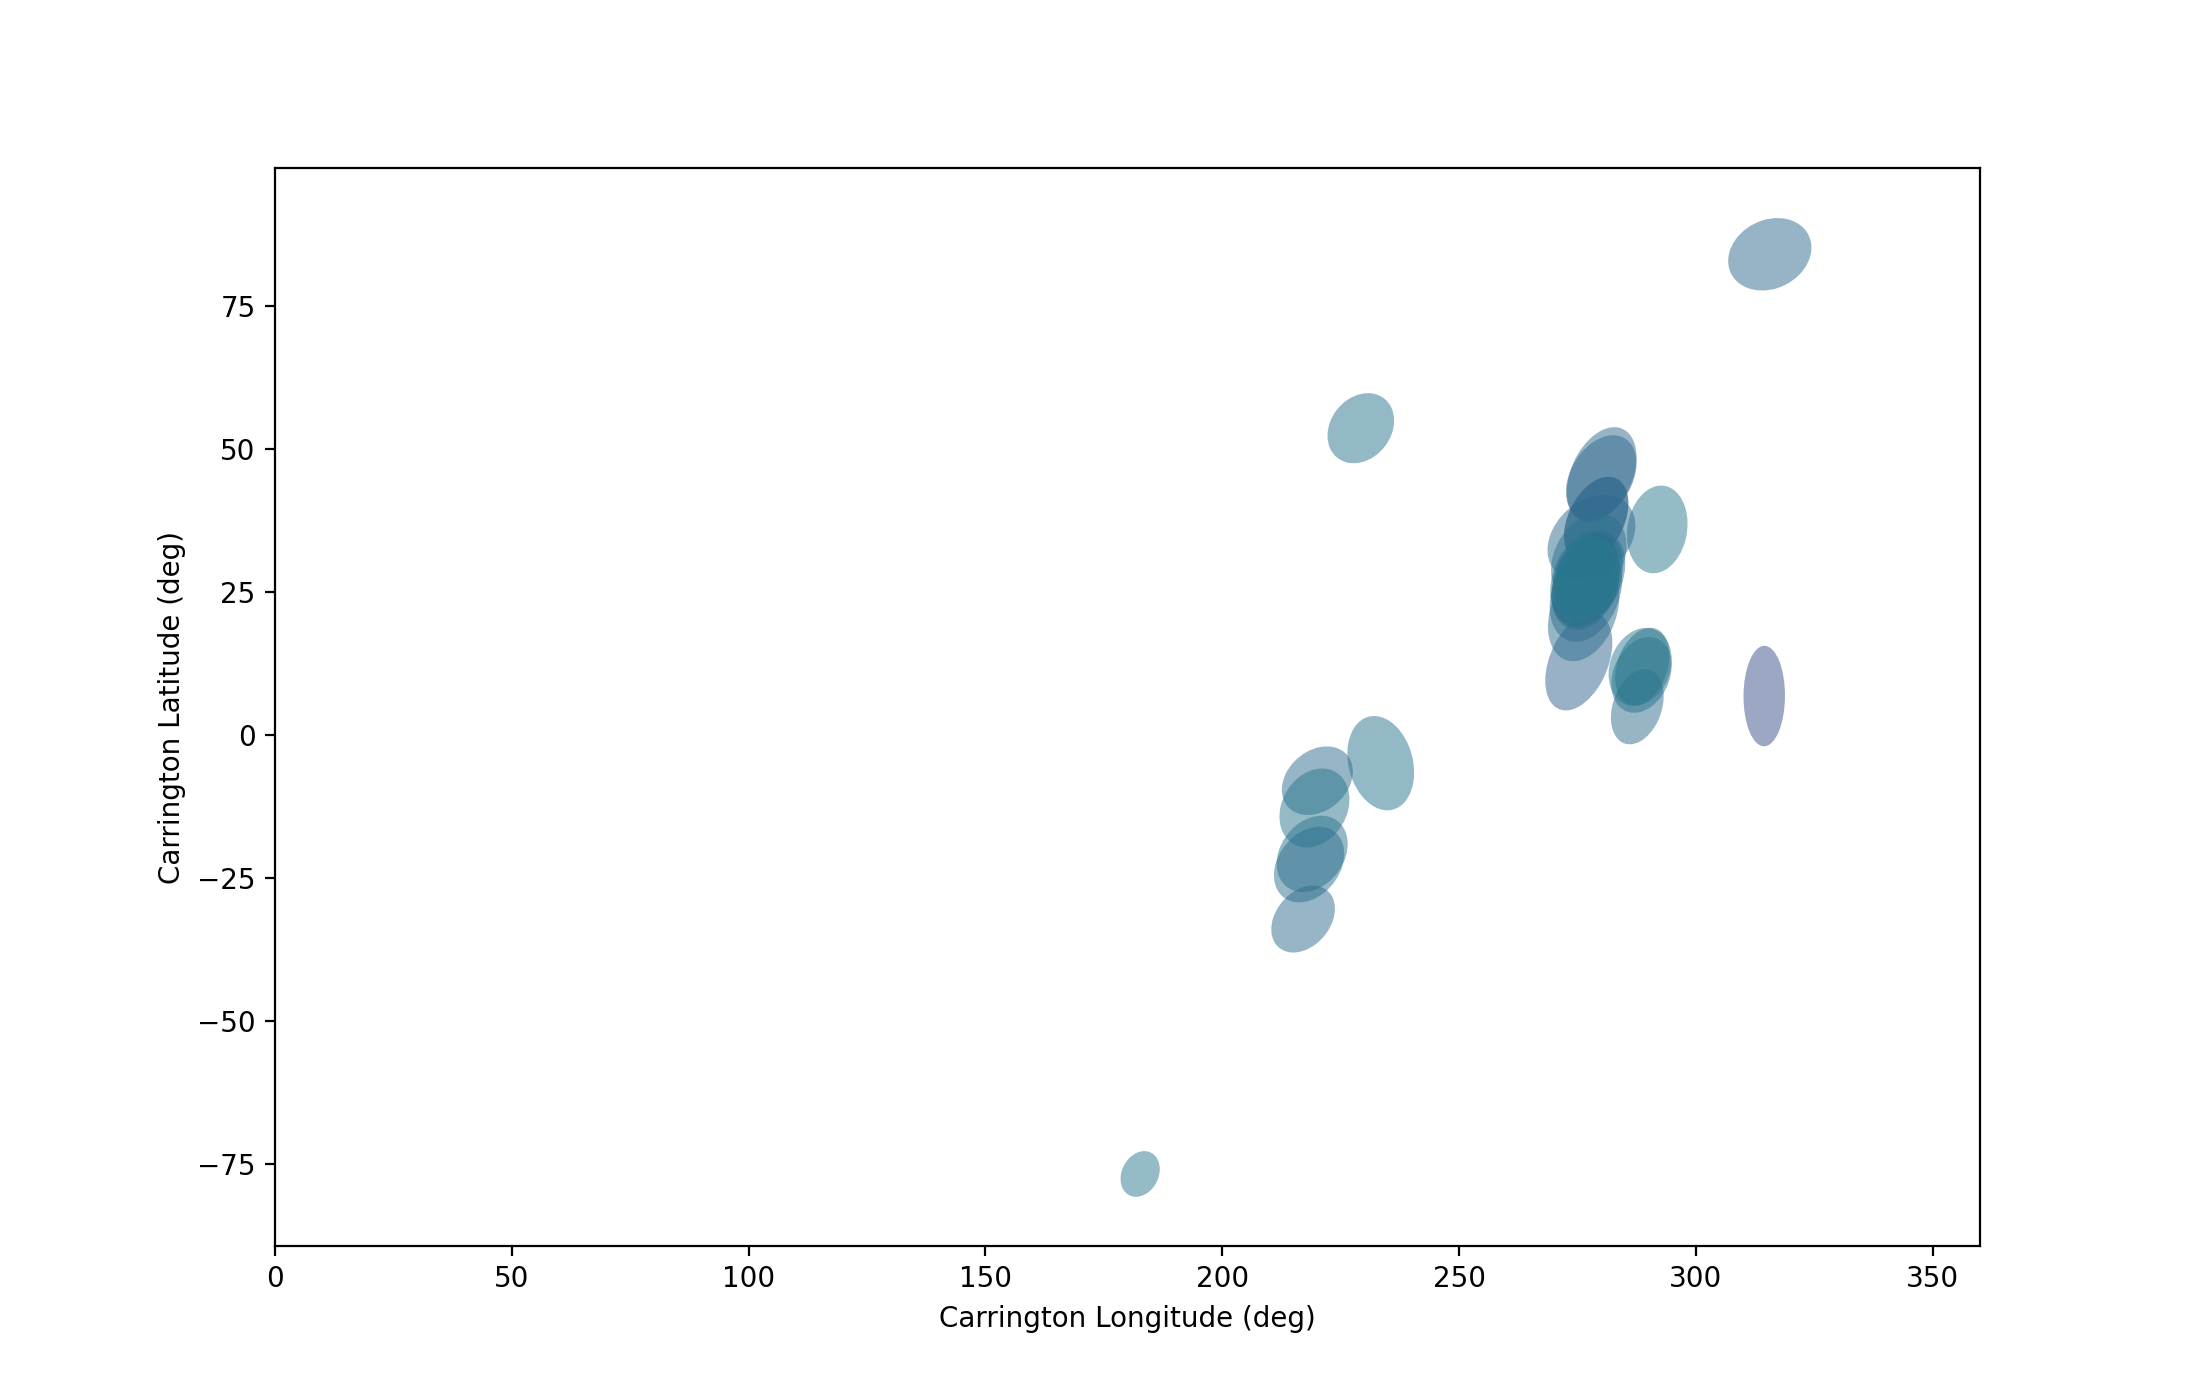
\includegraphics[width=\columnwidth]{burst_ellipses_carrington.png}
\caption[Synoptic AIA 193\AA  map overlayed with Type III radio bursts.]{A 193 \AA  AIA synoptic map where each fitted radio burst is overplotted. }
\label{fig:synoptic_bursts}
\end{figure}

\begin{landscape}
\begin{table}
\centering
\caption[Table of fitted burst parameters]{Table of fitted burst parameters for each of the 30 bursts described in Section \ref{sec:obsvtheory_method}. The units in each column are given. Here $I_0$ is the maximum intensity of the burst, $x_0$ and $y_0$ are the x and y  helioprojective coordinates of the burst, FWHM\textsubscript{x} and FWHM\textsubscript{y} are the burst sizes in the x and y direction and $\theta$ is the position angle of the fitted Gaussian.}
\label{tab:dataset}
\begin{tabular}{lcccccc}
\toprule
Burst Time & $I_0$ (arbitrary) & $x_0$ (arcsec) & $y_0$ (arcsec) & FWHM\textsubscript{x} (arcmin) & FWHM\textsubscript{y} (arcmin) & $\theta$ (degrees) \\
\midrule
2019-04-05T12:08:08.082 &   90333.34 & -1772.89 &   213.66 &    8.76 &   17.58 &  -26.59 \\
2019-04-07T12:02:28.512 &   83782.44 & -1924.03 &   411.53 &   10.28 &   14.48 &  -56.52 \\
2019-04-07T12:04:21.926 &  108123.57 & -1990.30 &   372.36 &   11.29 &   14.52 &  -66.65 \\
2019-04-07T12:15:07.681 &  160081.88 & -1677.12 &  1228.90 &   12.48 &   15.59 &  -43.79 \\
2019-04-07T12:30:59.620 &  120107.74 & -1896.80 &   165.35 &   10.01 &   14.02 &  -56.17 \\
2019-04-07T12:51:39.288 &   47916.36 & -1979.35 &   420.47 &   12.15 &   14.72 &  -67.42 \\
2019-04-08T12:00:15.636 &  117196.69 & -1310.37 &  1020.77 &   11.16 &   16.93 &  -63.68 \\
2019-04-08T12:00:15.636 &  117196.69 & -1310.37 &  1020.77 &   11.16 &   16.93 &  -63.68 \\
2019-04-08T12:06:40.505 &  316272.33 & -1579.55 &   818.51 &   13.12 &   18.67 &  -65.64 \\
2019-04-08T12:08:36.604 &   60696.79 & -1616.67 &   840.69 &   11.28 &   14.28 &  -50.02 \\
2019-04-08T12:22:34.290 &  171058.10 & -1380.68 &   643.10 &   13.59 &   18.40 &  -60.80 \\
2019-04-08T12:26:53.834 &  111428.17 & -1479.15 &   338.94 &   11.89 &   18.69 &  -58.46 \\
2019-04-08T12:29:00.334 &   77443.59 & -1341.21 &   533.82 &   13.33 &   18.65 &  -58.68 \\
2019-04-08T12:34:57.353 &  176944.04 &  -934.63 &   947.11 &   12.09 &   17.18 &  -71.76 \\
2019-04-08T12:35:35.437 &  277659.44 &  -902.94 &   931.06 &   12.39 &   18.46 &  -61.85 \\
2019-04-08T12:42:59.698 &  119228.99 & -1653.25 &   878.17 &   12.36 &   16.18 &  -60.06 \\
2019-04-08T12:47:06.994 &  155057.08 & -1381.63 &   723.48 &   13.58 &   18.22 &  -62.20 \\
2019-04-08T12:48:49.167 &  296662.11 & -1305.03 &   648.47 &   12.83 &   16.99 &  -61.59 \\
2019-04-08T12:50:26.643 &  129463.84 & -1331.87 &   924.36 &   13.61 &   19.59 &  -89.59 \\
2019-04-08T12:54:34.610 &  207041.12 & -1485.08 &   898.27 &   13.60 &   17.91 &  -71.72 \\
2019-04-08T12:59:24.856 &  177435.14 & -1473.30 &   768.77 &   12.85 &   15.54 &  -65.86 \\
2019-04-11T12:56:26.514 &  215905.79 & -1221.80 &  -105.80 &   13.30 &   17.15 &   -0.49 \\
2019-04-12T12:00:18.153 &  179265.16 &  -362.53 &   500.60 &   11.41 &   14.77 &  -87.46 \\
2019-04-12T12:04:55.480 &  130911.18 &     3.26 &   399.69 &   12.25 &   17.88 & -101.70 \\
2019-04-12T12:14:50.568 &   43288.32 & -1438.75 &  -549.49 &   12.04 &   16.08 &  -83.24 \\
2019-04-12T12:39:31.661 &   86016.46 & -1040.30 &  -146.83 &   11.04 &   15.73 &  -91.31 \\
2019-04-12T12:49:33.963 &   74776.61 &  -888.52 &  -202.43 &   12.60 &   15.84 &  -79.74 \\
2019-04-12T12:51:54.388 &  132627.29 &  -805.26 &  -338.33 &   11.73 &   16.05 &  -82.21 \\
2019-04-12T12:53:51.493 &  127718.17 &  -687.98 &  -436.28 &   10.29 &   14.56 &  -83.17 \\
2019-04-13T12:30:30.763 &  100613.83 &  -162.06 &  -766.36 &    7.21 &    8.98 &  -75.73 \\
\bottomrule

\end{tabular}

\end{table}
\end{landscape}

The size of each burst, is plotted against the distance from the disk centre in the x and y direction in Figure \ref{fig:fwhm_comp}. There is no obvious trend towards bigger/smaller bursts with increasing distance from disk centre and, most strikingly, in direct contrast to the prediction by \cite{Kontar2019} there is no trend in the aspect ratio of the bursts, which is expected to trend towards 1 near disk centre and $< 1$ near the limb. Figure \ref{fig:fwhm_hist} shows a histogram of FWHM\textsubscript{x} and FWHM\textsubscript{y}in the range of 6 to 20 arcmins. The mean size of the bursts is indicated by a vertical grey dashed line and is $11.86$ arcmin for FWHM\textsubscript{x} and $16.35$ arcmin for FWHM\textsubscript{y}. This is consistent with previous observations of type III bursts at similar frequencies \citep{Kontar2017, Murphy2021}.

\begin{figure}[ht]
\centering
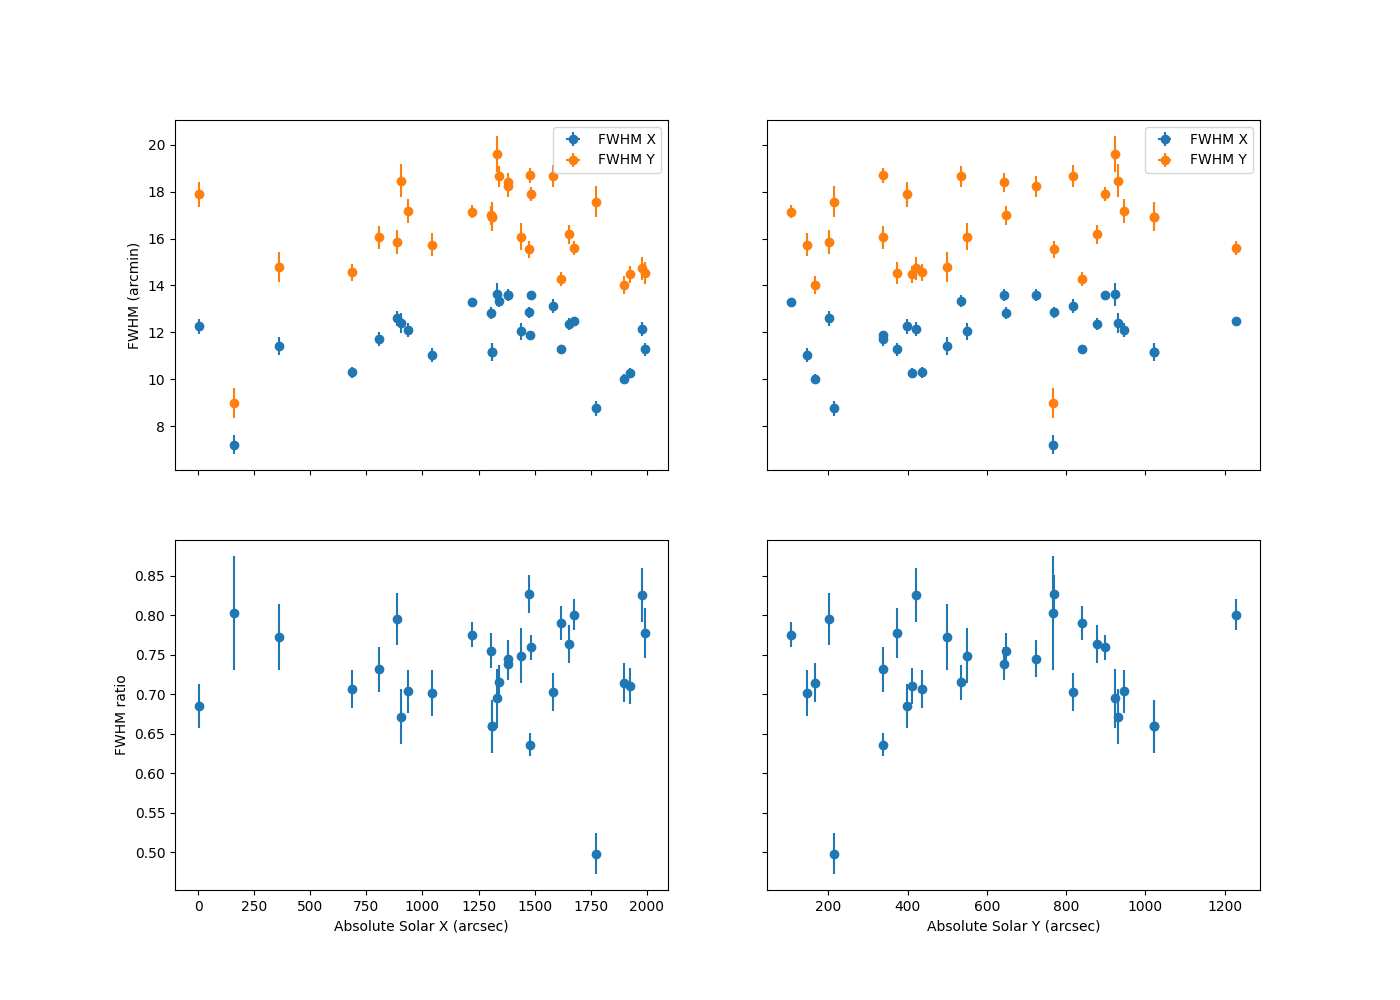
\includegraphics[width=\columnwidth]{fwhm_comparison.png}
\caption[Directly fitted Type III burst sizes as a function of position relative to disk centre.]{A comparison of the directly fitted Type III burst sizes and their location relative to the disk centre in the x and y direction. Top row, FWHM in x (blue) and y (orange) as a function of their distance from the disk centre in the x (left) and y (right) direction. Bottom row, same as above except showing the ``aspect ratio" of each burst.}
\label{fig:fwhm_comp}
\end{figure}

\begin{figure}[ht]
\centering
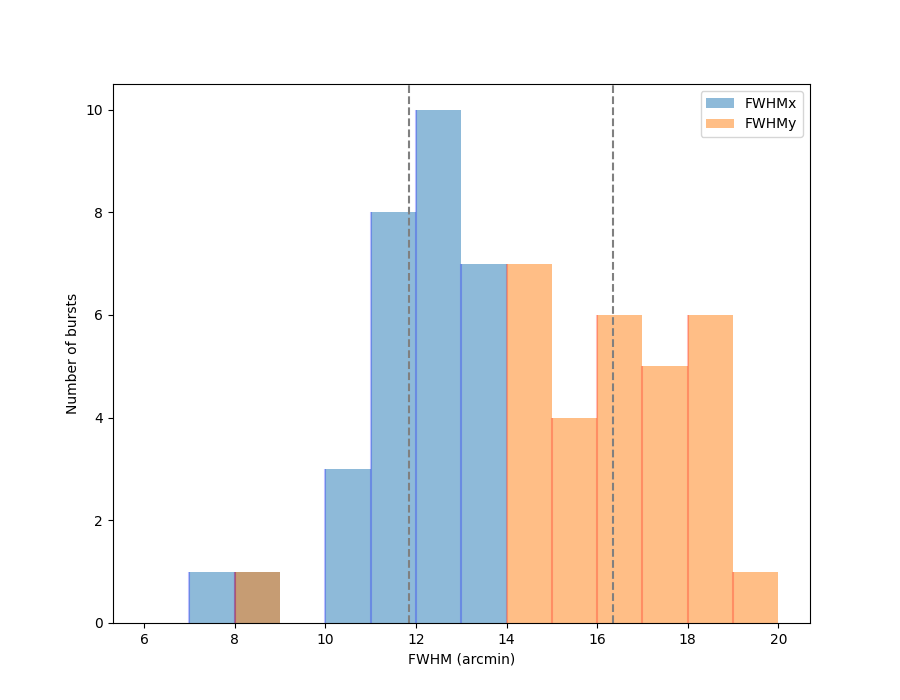
\includegraphics[width=\columnwidth]{burst_fwhm_histogram.png}
\caption[Histogram of type III burst sizes.]{Histogram of type III burst sizes. Bins are 1 arcmin wide and the vertical grey dashed lines indicate the mean value for FWHM\textsubscript{x} and FWHM\textsubscript{y}}
\label{fig:fwhm_hist}
\end{figure}

\section{Discussion}
\label{sec:obsvtheory_discussion}
The results given here are largely consistent with models of scattering through anisotropic density fluctuations in a spherically symmetric corona as presented by \cite{Kontar2019}. However, there is one major deviation in the results; no trend of source size vs heliocentric angle is evident in the data. The simplest, and perhaps most appropriate, answer to why this is the case is mentioned in the discussion of \cite{Kontar2019}. Since their work only analyses the path of photons from a point source, it is possible that Type III (and all other) radio bursts have an intrinsic source size. The total observed size then can be considered as the intrinsic size and the size due to scattering of a point source added in quadrature FWHM\textsubscript{total} = (FWHM\textsuperscript{2}\textsubscript{intrinsic} + FWHM\textsuperscript{2}\textsubscript{scattering})$^{1/2}$. Therefore, no trend in source sizes could suggest an intrinsic size greater than the size due to scattering. Interestingly, however, there appears to be a relationship in the orientation of the major axis of bursts being almost perpendicular to the radial line from solar centre. This suggest some form of aniostropic process... Another alternative is that the degree of aniostropy is in fact smaller than suggested by \cite{Kontar2019} and is closer to $\alpha = 0.5$, or even that it is not constant with time and or position (i.e. not axially symmetric as the MC method is based off of)
